\iffalse
\documentclass[12pt]{article}
\usepackage{graphicx}
\usepackage{amsmath}
\usepackage{mathtools}
\usepackage{gensymb}
\usepackage[latin1]{inputenc}
\usepackage{fullpage}
\usepackage{color}
\usepackage{array}
\usepackage{longtable}
\usepackage{calc}
\usepackage{multirow}
\usepackage{hhline}
\usepackage{ifthen}
\def\inputGnumericTable{}
\newcommand{\mydet}[1]{\ensuremath{\begin{vmatrix}#1\end{vmatrix}}}
\providecommand{\brak}[1]{\ensuremath{\left(#1\right)}}
\providecommand{\norm}[1]{\left\lVert#1\right\rVert}
\newcommand{\solution}{\noindent \textbf{Solution: }}
\newcommand{\myvec}[1]{\ensuremath{\begin{pmatrix}#1\end{pmatrix}}}
\let\vec\mathbf

\begin{document}
\begin{center}
\textbf\large{CHAPTER-7 \\ COORDINATE GEOMETRY}
\end{center}
\section*{Excercise 10.7.2.9}

1. Find the coordinates of the point which divides the line segment joining $\vec(-2,2) \text{ and } \vec(2,8)$ into four equal parts
\\
\solution\\		
\fi
Let 
\begin{align}
\vec{A}=\myvec{-2\\2\\},
\vec{B}=\myvec{2\\8\\},
\end{align}
Using section formula 
\begin{align}
\vec{R}_i&=\frac{\vec{B}+n\vec{A}}{1+n}
\end{align}

\begin{enumerate}

\item $n = 3$
    
\begin{align}
\vec{R}_1=
\myvec{
-1\\
\\
\frac{7}{2}\\
}
\end{align}

\item $n = 1$
\begin{align}
\vec{R}_2
=\myvec{
0\\
5
}
\end{align}

\item $n=\frac{1}{3}$
\begin{align}
\vec{R}_3
=\myvec{
1\\
\\
\frac{13}{2}\\
}
\end{align}

\end{enumerate}
See Fig. 
\ref{fig:chapters/10/7/2/9/Fig}
\begin{figure}[!h]
\begin{center}
   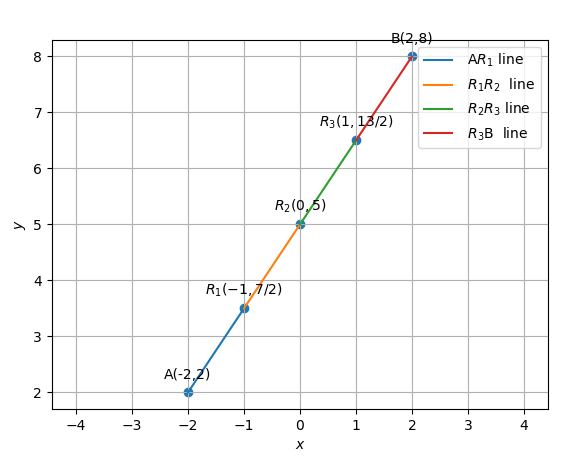
\includegraphics[width=\columnwidth]{chapters/10/7/2/9/figs/10.7.2.9.png}
\end{center}
\caption{}
\label{fig:chapters/10/7/2/9/Fig}
\end{figure}

